%%% MORITZ 2.5' %%%

\section{Doppelresonanz}
\subsection{Grundlagen: Optisches Pumpen}


\begin{frame}
\frametitle{Optisches Pumpen}
\setbeamerfont{myfont}{size*=45}
\usebeamerfont{myfont}

  \begin{figure}
    \centering
    \def\svgwidth{0.45\textwidth}
    \input{../img/termschema.pdf_tex}
    \caption{Termschema.}
\end{figure}
\end{frame}




\begin{frame}
\frametitle{Optisches Pumpen}

\begin{figure}[H]
\begin{center}
  \includegraphics[width=\textwidth]{../img/optPumpen.png}
  \caption{ca.}
\end{center}
\end{figure}
%TODO neues Bild mit Inkscape?

\end{frame}


\begin{frame}
\frametitle{Aufbau Doppelresonanz}

\setbeamerfont{myfont}{size*=80}
\usebeamerfont{myfont}
\begin{figure}
    \centering
    \def\svgwidth{\textwidth}
    \input{../img/aufbauDR.pdf_tex}
    \caption{Aufbau zur Messung der Doppelresonanz.}
\end{figure}

\end{frame}



%%% BEN 2.5' %%%

\subsection{Aufbau}
\begin{frame}
\frametitle{Aufbau}
  
\end{frame}

\subsection{Auswertung}
\begin{frame}
\frametitle{Auswertung}
  
\end{frame}